\chapter{Method of design}
  In this chapter, the design procedure will be described, and the choices we made will be clarified. The test-measurements is then explained in detail. During the design process we will use the models given for inductors and capacitors. We will use ideal resistors from the libraries in ADS.
  \section{DC Bias point at gate}
    The first step in designing a power amplifier is to choose the DC bias point, which will define the amplifier’s class of operation.We will be aiming for a deep AB class design because this gives a good compromise between gain, linearity and efficiency. This enables us to meet the required specifications as well as obtain good results with respect to the other performance parameters with no set requirements.
    We are using the ADS Design Guide called FET\_ IV\_ Gm\_ PowerCalcs, where we inserted the transistor as shown in figure~\ref{fig:fig_bias_sim}. From the design guide we used the I/V-plot to find the gate bias voltage that gives the desired quiescent drain current of 300mA, which will be used as bias point as this will be low in the class AB range $(0 < Ids < Imax/2)$. We may need to tweak the quiescent current when testing the real amplifier. The gate bias voltage that gives this quiescent current was found to be -2.6V.

  \begin{figure}[h]
	  \centering
	  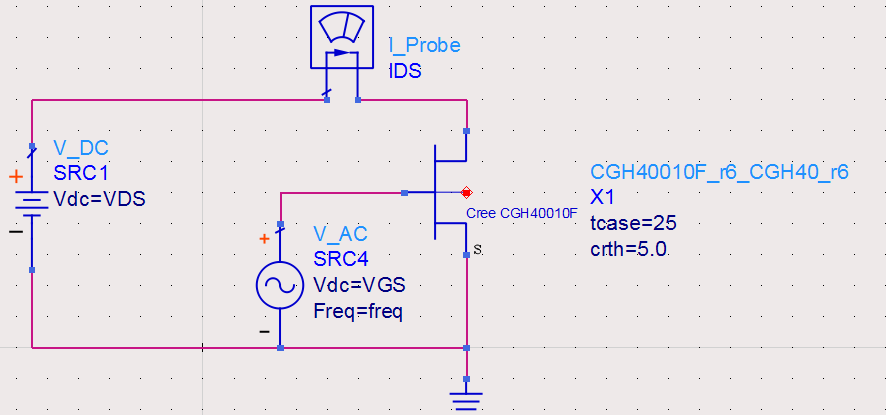
\includegraphics[width=0.75\textwidth]{img/IV_simulation}
	  \caption{Setup for bias-measurements}
	  \label{fig:fig_bias_sim}
  \end{figure}

  \section{Bias network}
  To ensure that the RF input does not affect the DC power supply, a quarter-wave transformer was used to present an infinite impedance in the 2.4GHz band when looking towards the DC power supplies from the RF signal pathways. The values were tuned to obtain optimal ac-block as seen from the transistor gate. In addition, a bank of lumped capacitors were used to prevent noise from the DC power supplies from entering the RF signal pathway as shown in figure~\ref{fig:Schem_Bias}. The same DC bias network was used for both the gate and drain DC bias voltage connections.
  
  \begin{figure}[h]
	\centering
	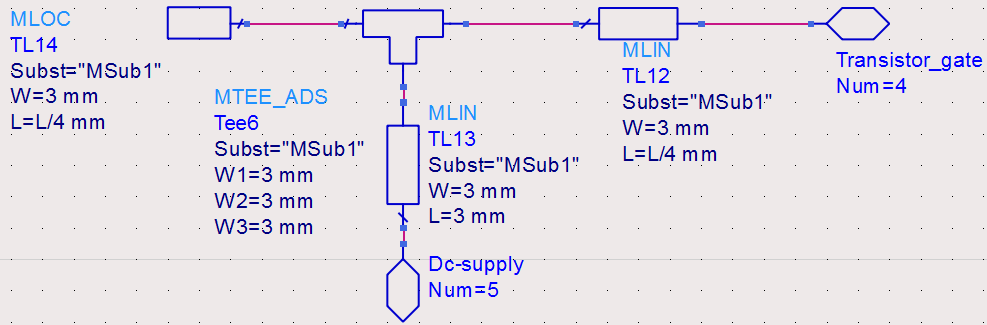
\includegraphics[width=0.75\textwidth]{img/Bias_network}
	\caption{Setup for bias-network}
	\label{fig:fig_bias_net}
  \end{figure}
  
  \section{Stability}
  To check if the amplifier is stable, we used the small-signal S-parameter simulations in ADS with added blocks for measuring the stability factors ($\mu$ and $\mu_{prime}$) on the input and output. According to the measurements, the amplifier is stable at higher frequencies, but at lower frequencies it is unstable. To remove the instabilities we will introduce losses at the lower frequencies, by adding a series RC element at the input, and a resistor at the DC bias feed point as shown in figure~\ref{fig:fig_stab_net}.
  \begin{figure}[h]
	\centering
	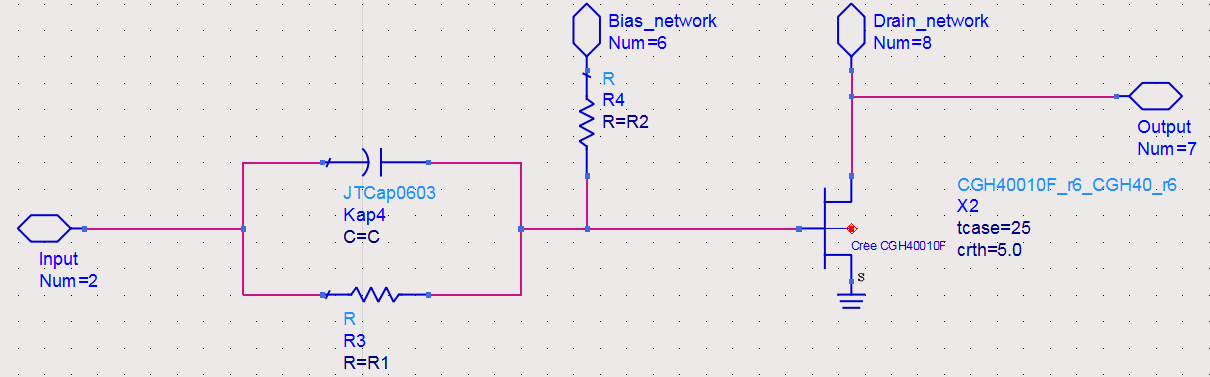
\includegraphics[width=0.75\textwidth]{img/Stability_network}
	\caption{Stability-network}
	\label{fig:fig_stab_net}
  \end{figure}
  The capacitor Kap4 and Resistor R3 presents a high impedance for lower frequencies, but for higher the capacitor is an effective short. The resistor R4 is introduced as a loss for all frequencies.
  
  The values C,R1 and R2 were found by using ADS’ optimization feature, with optimization goals for the stability factors ($\mu$ and $\mu_{prime}$) and the maximum available gain. The lowest value for the stability factors across the simulated frequency range from 0Hz to 6GHz was 1.05.

  \section{Matching}
  When stabilizing the amplifier, one of the goals for optimization was maximum available power. To achieve this power, one must match the input and output to 50 Ohm. To realise this without having to mount more components we designed a L-network consisting of an open circuit stub and a microstrip line as shown in figure~\ref{fig:fig_match_net}.
  \begin{figure}[h]
	\centering
	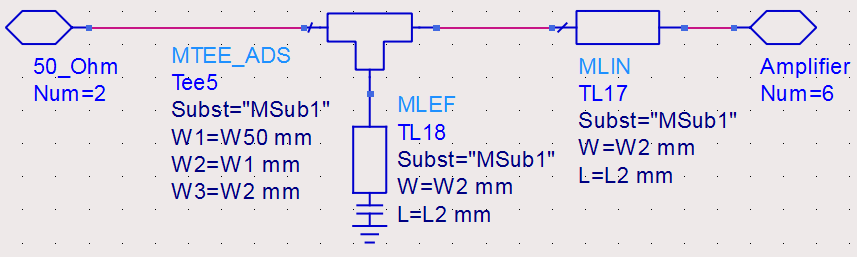
\includegraphics[width=0.75\textwidth]{img/Matching_network}
	\caption{Setup for matching the amplifier with 50$\Omega$}
	\label{fig:fig_match_net}
  \end{figure}
  The setup was used both on the input and output of the amplifier, and optimized for max power within the band.
  
  \section{Large signal simulation, one tone input signal}
  To run large signal simulation, a design guide called HB1TonePAE\_Pswp was used. In the design guide we checked the power added efficiency, the interpolated output spectrum and fundamental output power. We saw that power added efficiency was low, so we ran an optimization with increased power added efficiency and output power with 27dBm input as goals.
  
  \section{Large signal simulation, two tone input signal}
  To run large signal simulation two tone, a design guide called HB2TonePAE\_Pswp was used. In the design guide we checked the Power added efficiency, interpolated output spectrum and the output power with 27dBm as input. 
  
  \section{Layout and conversion to real components}
  Now that the design is complete, all components that are related to the layout will be added. This is done to make sure that the layout will fit within the predefined board size and that there is as few as possible steep transitions between different widths of microstrip line. The transistor was placed in the center of the board for heat sink mounting. Bends were used on the microstrips to fit the geometrical restrictions. The final schematic is shown in figure~\ref{fig:Schem_Input} and ~\ref{fig:Schem_Output}. The resulting layout is shown in figure ~\ref{fig:Layout}.
  
  \section{Tests with complete layout}
  After all physical changes were done, the amplifier as a whole was simulated to make sure the requirements were still fulfilled. A few tweaks with respect to line geometry was needed to obtain similar responses but the design passed the requirements given by the task.
  
  \section{Laboratory measurements}
  The goal for the measurements is to determine if the amplifier (DUT) passes the requirements given by the task or not. To do this we need to perform a small signal gain test, one-tone large signal test and a two-tone large signal test.
  \subsection{Small-signal s-parameters}
	\begin{figure}[h]
	  \centering
	  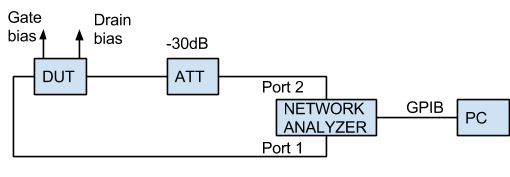
\includegraphics[width=0.75\textwidth]{img/Small_signal_meas}
	  \caption{Small-signal measurements setup}
	  \label{fig:fig_small_meas}
    \end{figure}
	As shown in figure~\ref{fig:fig_small_meas}, an attenuator was connected to the output of the amplifier to protect the network analyzer ports from excessive input voltages that could damage the instrument. The network analyzer was calibrated using a TOLS (through-open-load-short) calibration sequence.
  
  \subsection{Large signal one- and two-tone}
    \begin{figure}[h]
	  \centering
	  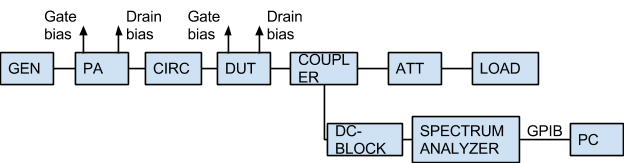
\includegraphics[width=0.75\textwidth]{img/Large_signal_meas}
	  \caption{Large-signal measurements setup}
	  \label{fig:fig_large_meas}
    \end{figure}
	We were at liberty to choose three set frequencies to perform the large-signal testing at. We chose the frequencies 2.35 GHz, 2.40 GHz and 2.45 GHz, because testing at these frequencies would give us the best prerequisites for determining if we had met the requirement specifications within the band of operation. As shown in figure~\ref{fig:fig_large_meas} there are several items that will introduce losses in the signal pathway, all of which must be subtracted from the measured power levels when analyzing the results in Matlab.

  